\documentclass[11pt]{article}
\usepackage[utf8]{inputenc}
\usepackage[english]{babel}
\usepackage{amsmath}
\usepackage{graphicx}
\usepackage{float}
\usepackage{lipsum}
\usepackage{multicol}
\usepackage{xcolor}
\usepackage{tabularx}
\usepackage{tikz}
\usepackage{booktabs}
\usepackage{float}
\usepackage{hyperref}
\usepackage{caption}
\usepackage{enumitem}


\newcolumntype{Y}{>{\centering\arraybackslash}X}
\usepackage[left=2.00cm, right=2.00cm, top=2.00cm, bottom=2.00cm]{geometry}
\title{AN2DL Reports Template}

\begin{document}

    \begin{figure}[H]
        \raggedright
        
\includegraphics[scale=0.5]{polimi.png} \hfill 
\includegraphics[scale=0.3]{airlab.jpeg}
    \end{figure}
    
    \vspace{5mm}
    
    \begin{center}
        % Select between First and Second
        {\Large \textbf{AN2DL - Second Challenge Report}}\\
        \vspace{2mm}
        % Change with your Team Name
        {\Large \textbf{ReLUctant}}\\
        \vspace{2mm}
        % Team Members Information
        {\large Alessandro Del Fatti,}
        {\large Matteo Garzone,}
        {\large Francesco Genovese} \\ 
        \vspace{2mm}
        % Codabench Nicknames
        {Kaggle: alessandrodelfatti,}
        {matteogarzone,}
        {frncscgnvs} \\
        \vspace{2mm}
        % Matriculation Numbers
        {270240,}
        {279709,}
        {307916} \\
        \vspace{5mm}
        \today
    \end{center}    
    \vspace{5mm}
    \begin{multicols}{2}
    \section{Introduction}
        This assignment focuses on the classification of low-magnification Whole Slide Images (WSIs) of human tissue into four distinct molecular subtypes associated with potential diseases. Specifically, the task involves identifying breast cancer subtypes. As better discussed in the experiment section, we followed the pipeline described by Liu et al. \cite{liu2022breast}, adapting their strategies to our dataset.
        
        \vspace{-5mm}

        \section{Data analysis and cleaning}

        \vspace{-2mm}

        % dataset composto da immagini e maschere
        Every sample of the given dataset is composed of two distinct components: the image itself and a mask delimiting the border of the cancerous portion of the cell.
        
        % immagini da pulire
        From a first analysis of the training set, we noticed that a subset of the images was provided dirty; In particular, they \textbf{were compromised} by significant artifacts: these images contained extraneous marker ink or \textbf{distinct greenish anomalies} (Shrek's face or green slimes). To avoid noise in the training phase, we implemented a custom filtering algorithm specifically designed to detect and reject contaminated slides automatically.
        
        % classi sbilanciate
        Another key aspect of the dataset is the \textbf{class imbalance}: the distribution of classes (representing the four breast cancer subtypes) were not uniform. Certain subtypes, such as Luminal A and Luminal B, were more prevalent, while Triple Negative samples were relatively underrepresented, as shown in the bar-plot in Figure \ref{fig:barplot}


        %%TODO EXPORT THIS TO SVG AND INCLUDE IT!
        \begin{figure}[H]
            \centering
            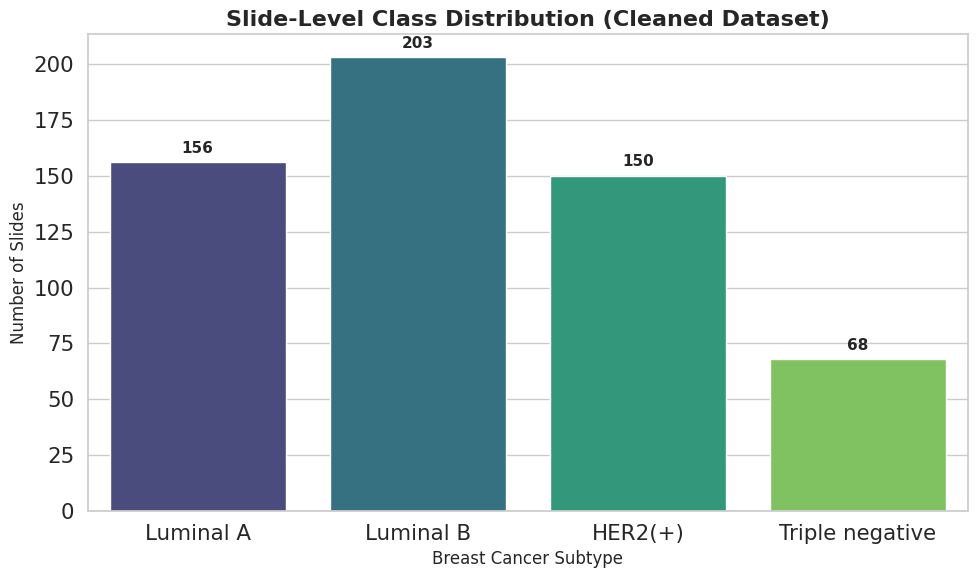
\includegraphics[scale=0.25]{barplot.png}
            \vspace{-0.3cm}
            \caption{Breast cancer subtypes distribution}
            \label{fig:barplot}
        \end{figure}
        \vspace{-1.0cm}
        \section{Method} 
        \vspace{-0.2cm}
        \subsection{Preprocessing Pipeline}
        \vspace{-2mm}
        \subsubsection{Normalization} 
        We initially implemented a standardization pipeline combining 
        \begin{itemize}[noitemsep,topsep=0pt]
            \setlength{\itemsep}{1pt}
            \setlength{\parskip}{0pt}
            \setlength{\parsep}{0pt}
            \item \textbf{Macenko Normalization} \cite{macenko2009method} 
            \item \textbf{Araujo Contrast Stretching} \cite{araujo2017classification}
        \end{itemize}
            to mitigate staining variations. However, qualitative analysis suggested that this approach could amplify artifacts in sparse tissue regions, leading to unnatural color saturation. Consequently, we also explored a raw data strategy using standard \textbf{Z-score normalization} during the embedding phase. This allowed us to compare the efficacy of the two normalization strategies.
        
        \subsubsection{Patches extraction:}
        We implemented a \textbf{mask-guided extraction} pipeline at different resolutions (we tried 224×224 and 256x256), partitioning the dataset at the slide level to strictly \textbf{prevent data leakage}. Patches were retained only if the given masks indicated significant tumor content ($\geq 1\%$). To implicitly augment the training data, we utilized a 50\% overlap, whereas validation patches were extracted without overlap to ensure unbiased evaluation.
        
        %% IDK, seems worth mentioning
        We also experimented with same-size, overlapping training and validation patch extraction to simplify the final \textit{K-Fold Cross Validation} experiments.
        \vspace{-6mm}

        \subsection{Pipeline architecture}
        To ensure faster training, we saved to disk the extracted patches and the feature bags generated by the foundation model. This way, we cut training time and optimized training resources.        
        \vspace{-4mm}
        
        \subsection{Data Augmentation}
        In the final version, by leveraging the \texttt{Phikon} foundation model, we omitted standard geometric augmentations. While earlier experiments with CNN architectures like \texttt{ResNet} and \texttt{DenseNet} (described in the next sections) necessitated heavy augmentation to achieve generalization, \texttt{Phikon} is trained using \textit{Self-Supervised Learning} (\textbf{SSL}) objectives. This training explicitly forces the model to learn feature representations that are \textbf{invariant} to global view changes, rotations, and color shifts, rendering additional synthetic augmentation redundant.
        \vspace{-4mm}
        \subsection{Training Strategy}
        \subsubsection{Loss Function}
        \vspace{-2mm}
        \textit{Categorical cross-entropy} with class weights computed for minority class loss weighting.
        We also experimented with different combinations of:
        \begin{itemize}[noitemsep,topsep=0pt]
            \setlength{\itemsep}{1pt}
            \setlength{\parskip}{0pt}
            \setlength{\parsep}{0pt}
            \item  \textit{Label Smoothing loss:} a custom made categorical cross-entropy extension that also maps class labels to properly-distanced floats rather than equally-distanced integers. 
            \item \textit{Focal loss:} a categorical cross-entropy extension designed to address class imbalance in classification tasks by giving higher weights to hard-to-classify data samples while down-weighting samples classified with higher confidence. 

            \item \textit{Contrastive Loss:} a self-supervised auxiliary loss that encourages the model to learn robust, discriminative features by maximizing agreement between differently augmented views of the same slide while pushing apart features from different slides: 
            % \vspace{-0.2cm}
            % \small{
            % $$\mathcal{L}_{\text{contrast}} = -\log\frac{\exp(\text{sim}(z_i, z_i^+)/\tau)}{\sum_{k=1}^{K}\exp(\text{sim}(z_i, z_k)/\tau)}$$
            % }
            % \vspace{-0.7cm}
        \end{itemize}
        \vspace{-2mm}
        \subsubsection{Regularization Techniques and optimization}
 
       We first used the \texttt{AdamW} optimizer during preliminary testing. Then, we evaluated \texttt{Lion}. While \texttt{Lion} converges faster than the alternative, it is much more unstable.

       To adjust to this instability, we found similar performance to \texttt{AdamW}, with faster convergence, experimenting with
       
    \begin{table}[H]
    \centering
    \footnotesize
    \resizebox{0.5\textwidth}{!}{%
        \begin{tabular}{lcc}
            \toprule
            \textbf{Hyperparameter} & \textbf{AdamW} & \textbf{Lion} \\
            \midrule
            \textbf{Min LR}        & $10^{-5}$    & $10^{-7}$ \\
            \textbf{Dropout}       & $10^{-2}$    & $10^{-2}$ \\
            \textbf{L1}            & $10^{-5}$    & $10^{-5}$ \\
            \textbf{L2 (WD)}       & $10^{-4}$    & $10^{-4}$ \\
            \textbf{LR WarmUp ep.} & 10 & 15 \\
            \textbf{Scheduler}     & ReduceLRoP   & CosineAnn \\
            \bottomrule
        \end{tabular}%
    }
    \captionsetup{justification=centering}
    \caption{Hyperparameter configurations}
    \label{tab:optimizer_comparison_transposed}
\end{table}

        \vspace{-1cm}
        \section{Experiments}
        \vspace{-0.2cm}

        \subsection{Architecture Evolution}
        We explored multiple architectures in our progression toward an optimal Multiple Instance Learning (MIL) solution:
        
        \textbf{1. CNN Baselines:} Initially, we experimented with standard CNN architectures (\texttt{ResNet18}, \texttt{ResNet50}, \texttt{DenseNet121}, \texttt{EfficientNetB0}) applied directly to the slides. Despite extensive data augmentation, the models lacked generalization capabilities on the \textit{test set} as the performance proved to be slightly better than a four-sided-coin toss.
        
        \textbf{2. Patch-Based ResNet:} We then adopted a patch extraction strategy with \texttt{ResNet18} as a feature extractor, followed by aggregation methods. While this improved performance, the model struggled to generalize on the patches.
        
        \textbf{3. MIL with Attention:} We transitioned to a Multiple Instance Learning framework using gated attention mechanisms to aggregate patch-level features. This allowed the model to learn which patches were most relevant for classification.
        
        \textbf{4. Transformer-Based MIL:} Our final architecture combines:
        \begin{itemize}[noitemsep,topsep=0pt]
            \setlength{\itemsep}{1pt}
            \item \textbf{Phikon} foundation model (768-dim features) for patch-level feature extraction
            \item \textbf{Extraction of geometric features from masks} using a geometric mask encoder (128-dim features)
            \item \textbf{Transformer encoder} (3 layers, 8 attention heads) for modeling patch relationships
            \item \textbf{Gated attention} mechanism for slide-level aggregation
            \item \textbf{LayerNorm} throughout for training stability with small batch sizes
        \end{itemize}
    
        \vspace{-4mm}
        \subsection{Further augmentation}
        \vspace{-2mm}

        After implementing the MIL pipeline, we experimented with different augmentation and noise injection techniques, both on the extracted patches and on the feature bags extracted from the foundation model.

        We experimented\footnote{In a different notebook, called \texttt{experiments.ipynb}} with stochastic \textbf{CutMix} patch extraction and Feature Bags \textbf{MixUp} from same-class and same-slide patches and related features with different degrees of probability; however, the foundation model proved to be robust to these changes, as performance did not improve from these trials. 
        \vspace{-5mm}
        \subsection{K-Fold Cross-Validation}
        \vspace{-2mm}

        To obtain robust performance estimates, we implemented stratified 5-fold cross-validation at the slide level, ensuring no data leakage between folds. The final submission used an ensemble of all 5 fold models, soft-averaging their predictions to improve robustness and reduce variance.
        
        \vspace{-5mm}
        \section{Results}
        \vspace{-2mm}
        As the challenge progressed, we tested new models and introduced new pipeline, augmentation and training improvements, also following suggestions provided in the \textit{Log Book}. 

        As Table \ref{tab:results} suggests, further modifications of the MIL Transformer model took us to the final K-fold experiment, which yielded the best performance. 

        \vspace{-4mm}
        \section{Discussion}
        \vspace{-2mm}

        \subsection{Strengths of Our Approach}
        \begin{enumerate}[noitemsep,topsep=0pt]
            \setlength{\itemsep}{1pt}
            \setlength{\parskip}{0pt}
            \setlength{\parsep}{0pt}

            \item \textbf{Foundation Model Leverage:} Using Phikon pre-trained on histopathology provided domain-specific features superior to \texttt{ImageNet}-pretrained models.
            \item \textbf{Advanced/experimental training:} Combination of focal loss, contrastive learning, different slide, patch and feature augmentation techniques addressed both class imbalance and feature quality.
            \item \textbf{Robust Aggregation:} Transformer + attention mechanism captures global slide context from related patches.
            \item \textbf{Ensemble Strategy:} K-fold ensemble with uncertainty quantification improved reliability and reduced prediction variance.

        \end{enumerate}

        \vspace{-3mm}
        \subsection{Limitations and Lessons Learned}
        \begin{enumerate}[noitemsep,topsep=0pt]
            \setlength{\itemsep}{1pt}
            \setlength{\parskip}{0pt}
            \setlength{\parsep}{0pt}
            \item \textbf{Augmentation Risk:} Aggressive augmentation can create unrealistic patterns that do not generalize.
            \item \textbf{Computational Cost:} Full-resolution patch extraction and feature computation required significant GPU resources and time.
            \item \textbf{Limited Interpretability:} While attention weights provide some insight into important regions, understanding \textit{why} the model makes specific predictions remains challenging.
        \end{enumerate}

        \vspace{-4mm}
        \section{Conclusions}
        
        %%%%%%%%%%%%%%
        Starting from standard CNN baselines, we moved toward a \textbf{MIL framework} to address the specific challenges of high-resolution tissue analysis and class imbalance.
    
        Our final solution effectively integrated the \texttt{Phikon} foundation model for \textbf{domain-specific} feature extraction with a \textbf{Transformer-based} aggregation mechanism, supplemented by geometri}c features derived from tissue masks. Crucial to our methodology was the implementation of advanced training strategies, including focal loss, to stabilize convergence on underrepresented classes. Experimental results shown in Table \ref{tab:results} demonstrate the potential of this approach. 
        
        \textbf{Future developments} should focus on multi-scale patch processing to capture broader contextual information beyond fixed resolutions. Additionally, further work is required to enhance model interpretability, ensuring that the attention mechanisms provide clinically meaningful insights into the morphological features driving the classification.
        %%%%%%%%%%%%%%        
    
    \end{multicols}

    \newpage
     % --- BIBLIOGRAPHY COMMANDS ---
    \bibliographystyle{plain} 
    \bibliography{references}

    \section*{Appendix}
           \begin{table}[H]
        \centering 
        \caption{Summary of Experimental Results and Model Progression} \label{tab:experiments}
        \begin{tabular}{lcc} 
            \toprule \textbf{Experiment Category} & \textbf{Validation F1} & \textbf{Public Test F1} \\ & (Mean $\pm$ Std) & (Best Recorded) \\ \midrule 
            CNN-Based Experiments & $0.2315 \pm 0.018$ & $0.2343$ \\
            Pretrained Foundation CNNs & $0.2640 \pm 0.027$ & $0.2706$ \\
            Patch-Based Training & $0.3310 \pm 0.023$ & $0.3038$ \\
            MIL Transformer Learning & $0.3695 \pm 0.016$ & $0.3650$ \\
            \textbf{K-Fold MIL Transformer} & $\mathbf{0.4210 \pm 0.067}$ & $\mathbf{0.3963}$ \\ 
            \bottomrule 
        \end{tabular}
        \label{tab:results}
        \end{table}
        
\end{document}

